\documentclass[11pt]{article}
\usepackage[margin=1in]{geometry}
\usepackage{graphicx,booktabs,amsmath,amssymb,microtype,xcolor}
\usepackage{longtable,array,calc,etoolbox,pifont,mdframed}
\usepackage[hidelinks]{hyperref}
\usepackage{caption}
\usepackage{authblk}
\usepackage[numbers,sort&compress]{natbib}
\captionsetup{font=small,labelfont=bf}
\setlength{\parskip}{2pt}
\newcommand{\rd}[1]{\textcolor{black!70}{#1}}
\providecommand{\tightlist}{%
  \setlength{\itemsep}{0pt}\setlength{\parskip}{0pt}}
\setlength{\emergencystretch}{3em}
\newmdenv[linewidth=0.8pt,linecolor=black!45,backgroundcolor=black!4,
          skipabove=8pt,skipbelow=8pt,innertopmargin=6pt,innerbottommargin=6pt]{redaction}

\title{\bfseries The geometry of single-cell foundation models:\\
what they inherit, what they add, and what shapes it}
\author[1,2]{Ihor Kendiukhov}
\author[3]{Logan Riggs Smith}
\author[4]{Thomas Dooms}
\affil[1]{Institute of Medical Genetics and Applied Genomics, University of T\"ubingen}
\affil[2]{Pivotal Research}
\affil[3]{Cambridge Boston Alignment Initiative}
\affil[4]{Goodfire}
\renewcommand\Authands{ and }
\date{}

\begin{document}
\maketitle

\begin{abstract}
\noindent
Single-cell foundation models are said to learn the geometry of cell state, and that geometry is
increasingly used to justify their use for target prioritisation and perturbation prediction. We ask
three questions of it across nine representations plus a model-free control: what does it look like,
is any of it the model's own, and what makes it take the shape it does.

\textbf{What they inherit.} Cell-level geometry is a re-description of the input. Measured end to end
on the cell cycle, full expression scores $0.929$, the model's own tokenised input $0.882$, and the
model $0.875$, so the tokeniser costs seven times what the transformer contributes. Against matched
expression baselines the models win 1 of 45, 0 of 36 and 0 of 20 comparisons; raw data completes a
deleted manifold region better than they do, and transfers across tissues better as well. Knowing this
makes an accurate anatomy more useful, and several standing assumptions turn out to be wrong: the cell-cycle manifold is a \emph{filled disk rather than a
ring}, it is \emph{flat}, its angle encodes phase while its \emph{radius} encodes cycling strength, and
it is \emph{continuous} rather than a few discrete states.

\textbf{What they add.} The gene-token table holds facts absent from every individual input.
MaxToki-1B places any of ${\sim}18{,}000$ genes on one of 22 autosomes at $0.880$ balanced accuracy
(chance $0.045$) under a 10-megabase neighbourhood holdout, against $0.720$ for the strongest
training-free factorisation of the same cells, and the model acts on it: steering a chromosome
direction raises the model's own predictions for that chromosome's genes at untouched positions,
positive for 132 of 132 chromosome $\times$ strength $\times$ seed combinations, and reproducing a
measured leukaemia karyotype at $r=+0.43$. A cell-sentence model given one gene symbol and no other
phase information places it correctly at AUROC $0.989$, while an anagram of the same letters scores
chance. This is a class of latent variable distinct from prior emergent-world-variable results, namely
a property of the \emph{vocabulary}, absent from any single input and orthogonal to the training
objective.

\textbf{What shapes it.} On synthetic corpora with planted ground truth, a model allocates
representational distance \emph{where its own output distribution turns over fastest}
($+0.160$ over control, $p=0.0041$, 8/8 seeds, localised to the manipulated arc in 5/5). Density does
not predict where the distance goes, and difficulty predicts it with the sign reversed. This
law predicts the one real-data geometry that is demonstrably the model's own: C2S gives extra
representational room to the G1$\to$S restriction point, the commitment step of the cell cycle.
Navigability is fixed separately,
by topology: since $\oint \mathbf{w}\cdot d\mathbf{x}=0$, a constant steering direction must stall a
quarter-turn into any closed manifold, which we verify analytically, synthetically, and in seven
representations.

Running through all three is a methodological point we make explicit and supply tests for: a manifold
visible inside a model is usually a re-parametrisation of one already present in its input, and telling
the two apart requires a competitor built from the same cells rather than a permutation null.
\end{abstract}

\section{Introduction}

Foundation models trained on single-cell transcriptomes
\citep{cui2024scgpt,theodoris2023geneformer,rosen2026uce,levine2024cell2sentence} are now proposed
for decisions with real consequence: which gene to target, what a perturbation will do, what a cell in
diseased tissue is. Much of the case for them rests on geometry. These models are said to organise
cells along developmental trajectories, around the cell cycle, and into lineage hierarchies. If that
geometry is the model's own, it is evidence of learned biology that can be read out, steered, and
trusted.

The trouble is that geometry is easy to find and hard to attribute. The dominant statistical structure
in transcriptomic data is that genes expressed together stay together, and almost any biological
category one might wish to claim, including cell type, cell state, pathway and phase, is largely
\emph{defined} by co-expression. A representation that faithfully re-describes its input will
therefore display all of that structure, and a probe will read it out at high accuracy, without the
model having learned anything a linear method on the raw data could not supply.

\paragraph{A manifold in a model is usually a manifold in its data.} Naming this failure precisely is
one of the things this paper is for. A model can display a manifold for two quite different reasons. It
may have built one, or it may be re-describing in new coordinates a manifold that was already in the
data. From inside the model the two cases look identical: the same clean low-dimensional structure, the
same high probe accuracy, the same interpretable axes, the same satisfying picture. Only one thing
separates them, and it is not visible in the picture: whether a competitor holding the same information
does as well. Reports of geometry in these models rarely run that comparison, so on
the evidence usually given, a published manifold is a re-parametrisation of the input rather than a
discovery about the model. The same worry has been raised from the language side:
\citet{prieto2026correlations} show that the circular arrangement of month words inside a model is
recoverable by running PCA on the co-occurrence statistics of the text itself, so the geometry is
inherited from the data's covariance. We treat the separation as a measurement problem, give the tests
that settle it (Section~\ref{sec:controls}), and apply them to every claim we make.

\textbf{This paper separates three questions that the field routinely runs together, and answers each
across nine representations.} \emph{What does the geometry look like?} We give an anatomy, done
carefully enough to overturn several standing assumptions. \emph{Is any of it the model's own?} We
answer against baselines built from the same cells and, where possible, given exactly the model's own
input. \emph{What makes it take the shape it does?} We answer on synthetic corpora where we plant the
answer, which lets us state a mechanism rather than a correlation. The organising finding is that the
answer splits by \emph{what is being represented}. A \textbf{cell's} state is determined by its own
input, and the model re-describes it. A \textbf{gene's} meaning exists only across the corpus, and the
model genuinely learns it. That boundary organises everything that follows.

\paragraph{Contributions.}
\begin{enumerate}\itemsep1pt
\item \textbf{An anatomy of the cell-state manifold} (\S\ref{sec:inherit}). It is a filled disk rather
than a ring, it is flat, it decomposes into angle-as-phase and radius-as-cycling-strength, and it is
continuous rather than discrete. Five independently trained models agree on the developmental axis at
held-out cosine $0.98$ to $0.998$. All of this structure is present in raw expression.
\item \textbf{Vocabulary-level facts that no input contains, and evidence they are used}
(\S\ref{sec:add}): chromosome decoded genome-wide beyond a training-free factorisation and validated
causally against an external karyotype; gene identity carrying cell-cycle phase with an
identity-destroying control; function beyond a co-expression-matched null; and composable, steerable
lineage-regulator geometry.
\item \textbf{A mechanism for how representational geometry is shaped} (\S\ref{sec:shape}): models
spend distance where their own output changes fastest, demonstrated with planted ground truth and
confirmed in a real model; a theorem that predicts when steering must fail and the operator that works
when it can; and a measurement showing that the trajectory arrives bent at layer 0 rather than being
built with depth, with 40\% of what has been reported as curvature turning out to be vector magnitude.
\item \textbf{A protocol for attributing geometry to a model rather than to its input}
(\S\ref{sec:controls}): six tests that separate a learned structure from a re-parametrised one, each
stated so that it can be applied to a published claim without rerunning the original study.
\end{enumerate}

\begin{figure}[t]
\centering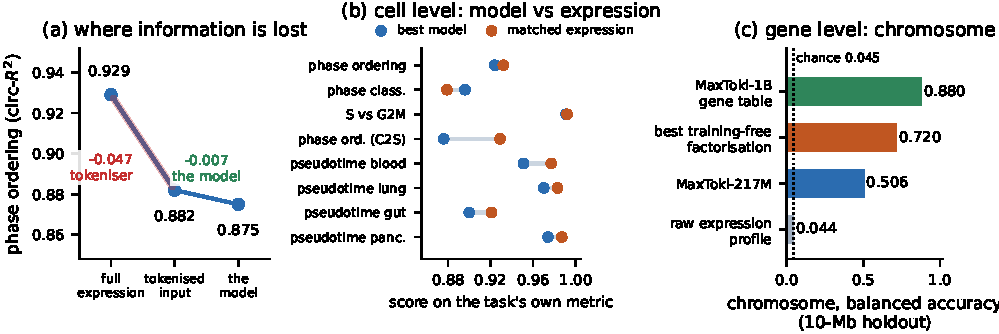
\includegraphics[width=\textwidth]{figures/fig1_two_regimes.pdf}
\caption{\textbf{Two representational regimes.} (a) On the cell cycle, information is lost at
tokenisation, not in the model: the transformer contributes $-0.007$ against the tokeniser's
$-0.047$. (b) Cell-level tasks, best model against a matched expression baseline. The two sit on top of
each other on every task, and expression is ahead on seven of eight. (c) At the gene level the model
holds a fact no single cell contains, beyond the strongest training-free factorisation of the same
cells.}
\label{fig:regimes}
\end{figure}

\section{Setup}

\subsection{Models and data}
Nine representations plus a model-free control, on shared substrates: scGPT \citep{cui2024scgpt}
(encoder, value-binned input; layer 11 and its native MVC head); Geneformer V1/V2
\citep{theodoris2023geneformer} (encoder, rank input); MaxToki 217M and 1B (Llama decoders, rank input,
untied \texttt{lm\_head}; all layers and both tables); STATE-SE/ST \citep{adduri2025state} and UCE-100M
\citep{rosen2026uce}, whose gene tokens \emph{are} frozen ESM-2 protein embeddings
\citep{lin2023esm2} and which therefore serve as the sequence control for vocabulary questions;
C2S-Scale 2B and 27B \citep{levine2024cell2sentence,rizvi2025c2sscale} (text LLMs over rank-ordered
gene name sentences); and raw expression. Substrates: Replogle K562 and RPE1 non-targeting controls
\citep{replogle2022genomewide} (cell cycle, $n=3{,}000$ each); Setty CD34$^+$ bone marrow
\citep{setty2019palantir}, fetal gut, lung airway and mouse pancreas \citep{bastidasponce2019pancreas}
(development); Tabula Sapiens \citep{tabulasapiens2022} (cell type and gene context). Cell-cycle phase
is scored with the standard marker sets \citep{tirosh2016melanoma,whitfield2002cellcycle}. Full details
in Supplement~A.

\subsection{Three questions}
We distinguish \textbf{readable} (a probe recovers it), \textbf{model-specific} (it beats a competitor
built from the same cells, given the model's own input where possible), and \textbf{causally used}
(intervening changes the model's own output, read through its native head, not a fitted probe).
These three are \emph{independent}, and all combinations occur in our data
(\S\ref{sec:controls}). They are commonly treated as a ladder, on which readable implies
model-specific and model-specific implies used. No step of that ladder holds.

\subsection{What kind of object each structure is}
``Manifold'' is used loosely for any low-dimensional structure. Most objects here are not manifolds,
and the distinction decides which operations are possible at all. A \emph{lookup}
(chromosome: 22 unordered classes) admits no path, only signed saturating shifts. An \emph{axis}
(paralogy) admits a fixed direction. An \emph{open tree} (pseudotime) needs a fixed direction plus
projection onto the local data tangent. A \emph{closed curve} (the cell cycle) makes a fixed direction
provably impossible (\S\ref{sec:stall}). A \emph{filled region} steers separately in angle and radius.
A \emph{fitted embedding} is a property of the fitting procedure, not of the model. We use
``representational geometry'' as the umbrella and name the type wherever we make a claim.

\section{Cell-state geometry is inherited from the input}\label{sec:inherit}

This section is about cells. \S\ref{sec:inherit} first asks who the cell-level geometry belongs to, the
model or the data, and then describes that geometry on the two structures these models are most often
said to build: the cell cycle and the developmental trajectory.

\subsection{The cell-level representation is a re-description of the input}
We start where the attribution question can be settled cleanly, because the answer changes how every
later result about cells should be read.

\paragraph{What is being tested.} Fix one task, one set of cells and one probe, then vary nothing but
the representation the probe reads from. The task is to recover where a cell sits in the cell cycle:
each of 3{,}000 K562 cells carries a phase angle computed from standard marker sets, and the probe is
a linear readout scored by circular $R^2$, which is $1.0$ for perfect recovery of the angle and $0$ at
chance. Give the probe the full expression vector and it scores what the data allows. Give it the
model's internal state and it scores what the model preserves. The informative rows are the ones in
between: representations holding exactly what the model was given and nothing more. C2S-Scale makes
those rows constructible, because its input is written out explicitly as the top-512 gene names in
rank order with magnitudes discarded, so a baseline can be handed \emph{exactly} the model's own
input. Reading the rows in order (Table~\ref{tab:accounting}) then separates the information lost when
a cell is tokenised from the change produced by running the transformer over it.

\begin{table}[h]\centering\small
\caption{\textbf{Information accounting on the cell cycle, end to end.} Each row is a linear readout of
cell-cycle phase from a different representation of the same 3{,}000 K562 cells. Reading down the
table, the loss from full expression to the model's tokenised input is $0.047$; the further loss from
that input to the model is $0.007$.}
\label{tab:accounting}
\begin{tabular}{lr}
\toprule
representation & phase ordering (circ-$R^2$) \\
\midrule
full expression, 6{,}546 genes with values & \textbf{0.929} \\
top-512 genes with values & 0.885 \\
top-512 set, binary presence, \emph{the model's input} & 0.882 \\
top-512 set $+$ rank, \emph{the model's input} & 0.868 \\
\textbf{C2S-2B L21, the model} & \textbf{0.875} \\
\bottomrule
\end{tabular}
\end{table}

The model sits \emph{on} a linear readout of its own input (Table~\ref{tab:accounting},
Fig.~\ref{fig:regimes}a). This replicates under a frozen cross-cell-line transfer (K562 $\to$ RPE1),
where the model scores $0.789$ against $0.792$ for a baseline matched on \emph{both} encoding and
gene-selection procedure, a paired $\Delta=-0.0022$, 95\% CI $[-0.0144,+0.0105]$. Matching only the
encoding gives a spurious ``the model adds information'' result ($\Delta=+0.0153$, CI excluding zero),
because a cell sentence draws its top-512 from the cell's \emph{full} panel while that baseline drew
from the shared genes. Both must be matched (Supplement~B.1). This is the protocol of
\S\ref{sec:controls} in miniature: the same experiment gives opposite verdicts depending on how the
competitor is built.

Three further lines agree (Fig.~\ref{fig:regimes}b). On matched-dimensionality benchmarks the models
beat expression in \textbf{1 of 45} cells and \textbf{0 of 36} (C2S); on developmental pseudotime
against a \emph{nonlinear} expression probe, \textbf{0 of 20}. Deleting a contiguous arc of a circular
trajectory from training, the model bridges the hole, but raw expression bridges it better at every
width, with the deficit growing from $-0.004$ at $30^\circ$ to $-0.027$ at $120^\circ$
(Supplement~B.3). And a pseudotime probe fitted on one tissue and applied unchanged to another
collapses for every representation: within-tissue Spearman $0.87$ to $0.95$, best cross-tissue $0.63$,
with 2 of the 3 pairs above $0.5$ won by raw expression (Supplement~B.4).

\emph{What follows from this.} The cell-level geometry belongs to the data. An accurate description of
it is still worth having, as a coordinate system on the expression manifold that is easier to compute
with than the raw counts. It is not evidence that the model learned biology. The next two subsections
do the describing, and \S\ref{sec:add} looks for the model's own contribution elsewhere.

\subsection{The cell cycle: the single-cell version of the day-of-week circle}
Language models place the days of the week on a circle, and place parts of the day on a second,
orthogonal circle \citep{engels2025circular}. That result is the template for a widespread claim in
single-cell biology, that these models likewise build a cell-cycle circle. The cell cycle is the one
cellular process everyone agrees is periodic, and a genuinely circular internal variable would license
a specific set of operations: read the phase, move along it, interpolate between phases. We asked what
that object actually is. Three widely repeated descriptions of it turn out to be wrong.

\paragraph{It is a filled disk rather than a ring.} A ring and a disk support different operations, so
the difference is not cosmetic: on a ring, radius carries nothing and every cell is at the same
distance from the centre; on a disk, radius is a second variable to read and to steer. Calibrated
against synthetic ground truth (Fig.~\ref{fig:anatomy}a), we report two statistics: the coefficient of
variation of the radius, and the fraction of cells lying inside half the median radius. A planted ring
gives $0.15$ and $0.000$; a planted disk gives $0.35$ and $0.126$. Observed: C2S-2B $0.38$ and $0.108$,
C2S-27B $0.38$ and $0.110$, raw expression $0.42$ and $0.122$. All three match the disk. Persistent
homology inside the fitted phase plane agrees ($H_1=0.227$ against a matched-covariance null
$0.251\pm0.063$, $z=-0.4$). Earlier low-dimensionality statistics were computed on bin centroids, which
describes the fitted summary, not the cells.

\paragraph{It is flat.} Curvature is what would make a cell-cycle representation more than a rotated
copy of a plane in the data, so its absence is worth establishing. The loop lies in a fixed linear 2-plane in every
representation, and $H_{\text{flat}}$ is never rejected (scGPT out-of-plane rotation $22.7^\circ$
against a planar-circle null $25.6\pm2.3$, $p=0.905$). Two consequences: a two-component linear
readout loses nothing, so nonlinear embeddings of the cell cycle add only visual appeal; and the stall
result of \S\ref{sec:stall} cannot be blamed on a difficult ambient shape, because there is none. This
is a statement about the cell-cycle loop alone. The \emph{developmental} trajectory does bend, and
\S\ref{sec:curv} measures by how much.

\paragraph{Angle is phase; radius is cycling strength.} This is where the day-of-week analogy pays off
most directly. In language models the day-of-week circle sits orthogonal to a parts-of-day circle, so
two different time variables occupy two clean, separable subspaces. The same two-factor structure holds
here. Phase programmes load on the angle at ${\sim}15\times$ the rate of non-phase programmes, and
cycling \emph{strength} is the only covariate with meaningful radial loading ($R^2=0.414$ radial
against $0.040$ angular; Fig.~\ref{fig:anatomy}b). A cell arrested in G1 and a cell cycling hard
through G1 sit at the same angle and different radii. Anyone reading phase out of one of these models
should read the radius too, because a low-radius cell has a phase estimate that means very little. Raw
expression shows the same split more strongly ($0.529$), so this structure is inherited as well.

\paragraph{It is continuous, and here the analogy breaks in the cell cycle's favour.} A week has seven
days and nothing between them. The language-model structure is seven \emph{discrete} points that happen
to be arranged on a circle, so a state one third of the way from Tuesday to Wednesday has no referent,
and the circle is a convenient layout for a categorical variable more than it is a manifold. A cell
one third of the way from S to G2M is an ordinary cell. Whether the models treat it that way is a
separate question, and the discrete answer is available to them: G1, S and G2M could sit as three
attractors with jumps between them, which would make interpolation meaningless and steering a matter
of hopping between basins. They do not. Three tests scored 0 (continuous) to 1 (discrete) give
behavioural interpolation $0.17$, metric profile $0.10$ and occupancy $0.00$
(Fig.~\ref{fig:anatomy}c): no empty regions around the loop, no jump in the metric, and interpolating
two cell states while reading the model's own marker logits moves the output gradually through
intermediate phases, with the intermediate state a genuine mixture. The model is, if anything,
\emph{more} uniform around the loop than the biology.

That interpolation test is the one that exposes \emph{activation plateaus} in language models, where
moving from one input sequence to another leaves the output almost unchanged along most of the path
before a sudden change part way through \citep{shinkle2025plateaus}. Those plateaus sharpen with depth
and follow the input-output sensitivity of the MLPs. We ran the equivalent interpolation here and got
the opposite on both counts: no plateau, and a plateau statistic that \emph{weakens} with depth
($0.179 \to 0.115 \to 0.056$ across layers 9, 15 and 21). Supplement~B.6 gives a falsifiable account,
namely that a plateau needs a discrete output alphabet, and a graded distribution over hundreds of
marker genes offers no cliff to form one. The two observations point the same way: the language-model
feature is discrete and the cell-cycle coordinate is not.

So the cell-cycle object is closer to a manifold in the strict sense than the language-model structure
that motivated looking for it. It is a continuous angular coordinate with no privileged points, lying
in a plane, carrying a second continuous coordinate that is also meaningful. The day-of-week circle is
a categorical variable wearing a circle's clothes.

\paragraph{Where the circle comes from.} On both sides of the analogy it comes from the data.
\citet{prieto2026correlations} take the months of the year, show that month words carry cyclic
co-occurrence statistics in text, and recover the same circle from a PCA of those statistics as from a
PCA of the learned weights; they call such structures inherited from data statistics. Every anatomical
property above behaves the same way here. Raw expression matches the disk calibration
($0.42$ and $0.122$), carries the angle-radius split more strongly than the models do ($0.529$ against
$0.414$), and supports the phase readout better ($0.929$ against $0.875$). Two different domains, two
different model families, and the same conclusion about where a reported circle comes from.

\paragraph{What the four results give a reader.} Read together, they say the cell-cycle object is a flat,
filled, continuous disk with two readable coordinates, and that it belongs to the expression data. That
is a usable description: it says which readouts are meaningful (angle and radius, jointly), and it
already forecasts the steering result of \S\ref{sec:stall}, because a closed loop is exactly the
topology on which a constant steering direction is guaranteed to fail.

\begin{figure}[t]
\centering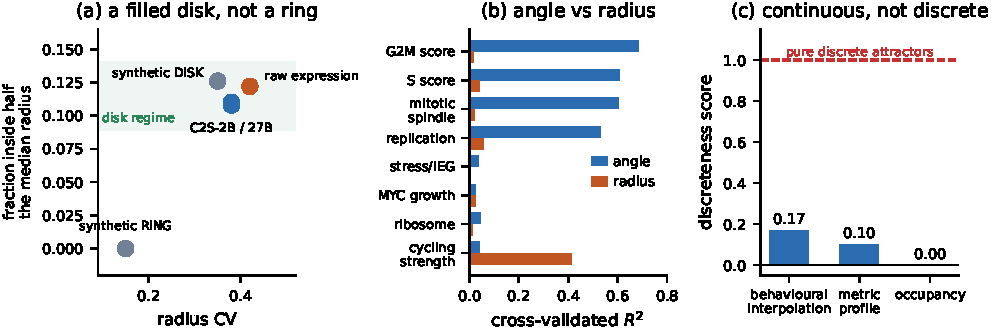
\includegraphics[width=\textwidth]{figures/fig2_anatomy.pdf}
\caption{\textbf{Anatomy of the cell-cycle manifold.} (a) Against synthetic ring and disk calibrations,
every representation, including raw expression, matches the disk. (b) A clean two-factor decomposition:
phase programmes load on the angle, cycling strength on the radius. (c) Continuity scores; 1.0 would be
discrete attractors.}
\label{fig:anatomy}
\end{figure}

\subsection{The developmental manifold: the object every steering claim rides on}
The cell cycle is closed and periodic. Development is the other shape these models are asked to
represent, and the shape with commercial consequences, because fate prediction, in-silico
differentiation and target ranking are all operations on a developmental trajectory. Its geometry
decides which of those operations can work at all, which is why we measure the shape before measuring
the performance.

Pseudotime is decodable everywhere (full-space linear $R^2$ $0.78$ to $0.97$ across 20 model $\times$
tissue cells). The local tangent \emph{rotates} along the trajectory, with $\theta_{\text{far}}$ of
$48$ to $113^\circ$ between the first and last pseudotime quintile, exceeding a heteroscedastic
residual-permutation null in \textbf{16 of 16} cells. The object is therefore a branching tree of
locally-linear segments, not one straight axis, and that single fact is what forces the operator
of \S\ref{sec:operator} to be local: a direction fitted globally points the wrong way by up to
$113^\circ$ at the far end of the trajectory it was fitted on.

\textbf{Five independently trained models agree on the developmental axis}, at held-out CCA-mapped
gradient cosine $0.9804$ to $0.9975$ across 20 ordered pairs, against a random-rotation null at $0.36$.
Models trained by different groups on different corpora with different objectives converge on the same
direction, which is strong evidence that the direction is a property of the biology they were all
trained on. Local intrinsic dimension falls as cells mature ($\rho=-0.31$ to $-0.75$), a potency
gradient, though a counts baseline reproduces it.

Pretraining does pay in one narrow place, which we state precisely because it is the exception to the
rest of \S\ref{sec:inherit}: endpoint targeting on hard, low-headroom trajectories (mouse
pancreas endpoint purity $0.207 \to 0.569$, with 4 of 4 models beating expression; lung $0.599 \to
0.862$, 4 of 4), and making trajectories \emph{linearly} readable, a real gain that dissolves against a
nonlinear probe (Supplement~B.5). The pancreas gain concentrates in the rare fates, which is where a
pretrained prior would be expected to help.

\emph{What follows from this.} The developmental object is a tree of locally-linear segments whose
tangent turns by up to $113^\circ$ from one end to the other, and five independently trained models
agree on where it points. Anything that treats it as a single global direction is therefore mis-specified
by construction, which is the failure \S\ref{sec:operator} diagnoses and repairs. This closes the cell:
the geometry is the data's, we now know its shape, and we know which operations that shape permits.
\S\ref{sec:add} asks whether these models add anything at all, at a different level.

\section{Gene-vocabulary facts the models add}\label{sec:add}

\S\ref{sec:inherit} closed off the cell: the geometry is inherited, with the narrow exception of
endpoint targeting on rare fates. The next question is whether there is any level at which these models
add something outright.

Our measurements do not explain \emph{why} the cell level came out that way, and we do not claim it had
to. What they do is suggest where to look next. A cell's state turned out to be largely recoverable
from that cell's own expression vector, and nothing the models did improved on that recovery. A gene's
meaning differs in one concrete respect: it is not present in any single cell and can only be assembled
across many of them, so a single-cell baseline has nothing to offer there. That makes the gene level
the natural place to look for a contribution from pretraining. It is a hypothesis, not a deduction, and
this section tests it. It holds.

\subsection{Chromosome membership, genome-wide}
We want a property that is unambiguously absent from every input, so that a positive result cannot be
explained by re-description. A gene's chromosome is such a property. It appears in no cell's expression
vector. It is recoverable only by aggregating co-occurrence across cells, because genes in the same
chromosomal neighbourhood tend to be co-regulated. It is also irrelevant to the training objective, so
nothing pushes a model to represent it.

\paragraph{Decoding.} A 22-way classifier on the gene-embedding table, split over genes, under
GroupKFold with \textbf{10-megabase genomic blocks} so that a gene's entire neighbourhood, including
duplicates, tandem arrays and TADs, is held out together and the gene cannot be placed by recognising a
near-identical twin: MaxToki-1B $\mathbf{0.880}$, strongest training-free factorisation $0.720$,
MaxToki-217M $0.506$, raw expression profile $0.044$, chance $0.045$ (Fig.~\ref{fig:regimes}c).
Permuted labels give $0.045$ and random-vector embeddings $0.042$; removing HOX and the protocadherin
array changes nothing; holding out whole token-ID blocks retains 96\%, so this is not tokeniser
adjacency; embedding norm alone predicts at chance. ESM-2 reaches $0.19$ on a random split but
\textbf{collapses to $0.07$} under the holdout (Fig.~\ref{fig:chrom}a), because its signal was
tandem-duplicate family resemblance. That collapse is the natural experiment separating sequence from
locus, and it is why the sequence control has to be run under the same holdout as the model.

\paragraph{Two limits.} Only the 1B clears the factorisation; the 217M falls short of
it. And on a \emph{label-free} retrieval test over gene pairs ${\ge}20$\,Mb apart the ranking
\textbf{inverts}, with the factorisation scoring $0.565$ against both models' $0.529$. The model's
margin is what a supervised probe extracts; the raw geometry is no more accessible.

\paragraph{Causal use.} Readability alone would leave this a curiosity, so we asked whether the model's
own computation uses the variable. Adding a chromosome-C direction to a random half of a cell's gene
tokens raises the model's own predicted probability of chromosome-C genes at the \emph{other,
untouched} half. Positive for \textbf{132 of 132} chromosome $\times$ strength $\times$ seed
combinations in the 1B (116/132 in the 217M); a norm-matched random push is flat; the response is
dose-monotone (Fig.~\ref{fig:chrom}c). This is read through the model's native next-gene logits rather
than a fitted probe. \textbf{External validation:} the same directions reproduce a measured aneuploid
karyotype's chromosome-level signature at $r=+0.43$, against a shuffled-karyotype control at
${\approx}0$.

\paragraph{Where the variable lives.} The variable is strong in the vocabulary tables ($0.516$ output,
$0.453$ input) and decays monotonically to $0.088$ by the last layer with no rebound; the 1B shows the
same pattern more sharply ($0.813 \to 0.066$ at matched width, retaining 8\%; Fig.~\ref{fig:chrom}b).
Steering works at the input embedding ($+0.0801$, 22/22) and is indistinguishable from zero by layer 5.
\emph{A variable can be functionally important while remaining undetectable as a feature at depth},
which is a caution for any layer-sweep study that reports the last layer only. We also tested the
mechanism usually assumed for this, attention between same-chromosome genes, and the data rule it out:
across 11 layers $\times$ 8 heads, same-chromosome gene pairs show \textbf{no attention enrichment}
once rank-distance is matched, with 0 of 88 heads significant and the strongest head changing identity
and flipping sign between samples. The causal effect is real; the route runs through the embedding
table, not through chromosome-sorted attention (Supplement~C.1).

\begin{figure}[t]
\centering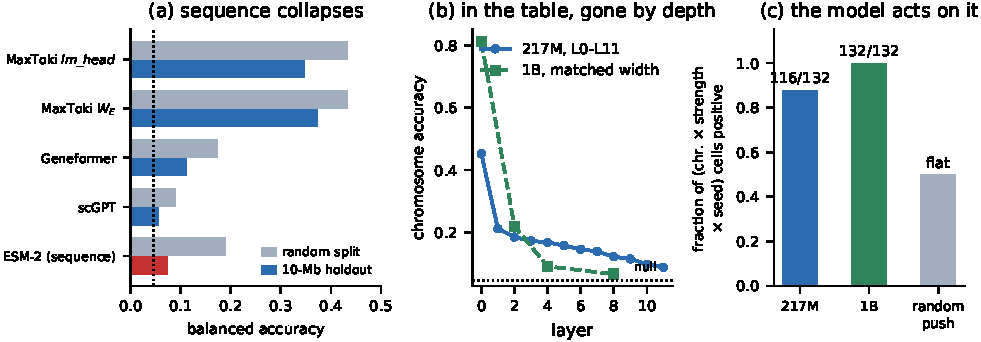
\includegraphics[width=\textwidth]{figures/fig3_chromosome.pdf}
\caption{\textbf{Chromosome membership.} (a) Under a 10-Mb neighbourhood holdout the model retains 78
to 85\% of its random-split accuracy, Geneformer 51\%, scGPT 24\%, and the ESM-2 sequence control
collapses to 20\%. (b) The variable lives in the table and the earliest
layers. (c) Steering is positive for every chromosome, strength and seed in the 1B.}
\label{fig:chrom}
\end{figure}

\subsection{A gene's identity carries its cell-cycle phase}
Chromosome shows that a corpus-level fact can sit in the table. The obvious follow-up is whether such
facts are ever \emph{biological}, or whether the table only holds bookkeeping. Here the test is the
strongest available for locating knowledge in the weights rather than the prompt, because the prompt is
stripped of the answer. Take a real cell, remove \emph{every} cell-cycle gene so the input carries no
phase covariance, insert \textbf{one gene symbol} at a fixed rank, and read which pole of the real-cell
phase circle the state lands on (Fig.~\ref{fig:surface}). Human \texttt{CCNB1} scores AUROC
$\mathbf{0.989}$ ($p=0.0002$, $40.7^\circ$ separation), while the \textbf{anagram} \texttt{NBCC1}
scores chance ($0.511$, $p=0.43$). The effect survives residualising on symbol length, abundance and
detection rate ($0.908$, $p=5\times10^{-5}$) and holds for 30 of 31 exact length-matched pairs
($p=3\times10^{-8}$).

\emph{Scope.} What transfers from the day-of-week result in language models is the
\emph{shape of the evidence}: a minimal prompt, an identity-destroying control, and structure that
survives both. The strength of the claim does not transfer. This is a two-class axis with a compressed
$40.7^\circ$ arc, offset from where real cells sit. ``The model knows \texttt{CCNB1} is mitotic'' is
supported. ``The model has an internal clock it can place any gene on'' goes beyond what we measured.

\begin{figure}[h]
\centering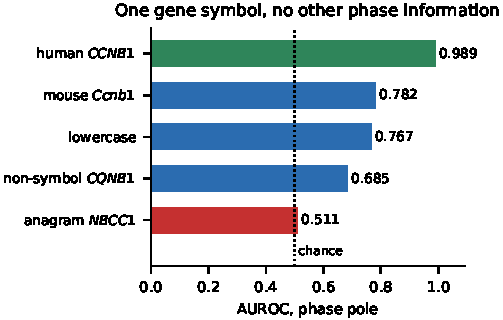
\includegraphics[width=0.48\textwidth]{figures/fig4_surface_forms.pdf}
\caption{\textbf{A surface-form ladder.} Five inputs, identical except for the single gene symbol
inserted: human \texttt{CCNB1} $0.989$, mouse \texttt{Ccnb1} $0.782$, lowercase $0.767$, the non-symbol
\texttt{CQNB1} $0.685$, and the anagram \texttt{NBCC1} $0.511$. Accuracy falls monotonically as the
symbol moves away from a real human gene name, and the anagram, which preserves every letter, sits at
chance.}
\label{fig:surface}
\end{figure}

\subsection{Function, paralogy, and lineage switches}
If the vocabulary table is a genuine store of corpus-level knowledge, the knowledge in it should not
stop at chromosome and phase. Three further probes ask how far it goes, and each is paired with the
baseline that could explain it away.

\textbf{Function beyond co-expression.} In C2S-Scale, same-function gene pairs are closer than
different-function pairs \emph{within matched co-expression and abundance bins}: $\Delta\cos$ of
$0.044$ to $0.062$, $z=3.9$ to $6.6$ against 200 co-expression-matched label permutations. This is one
of very few results here that clears a co-expression-matched null, not merely a permutation null, which
is the distinction \S\ref{sec:controls} is about.

\textbf{Paralogy as a composable coordinate.} Leaving one entire HOX cluster out, the paralog
coordinate transfers to it at held-out $\rho=+0.833$, with the correct sign in 4 of 4 clusters
($p=0.005$). Word2vec-style arithmetic works: \texttt{HOXA9} $-$ \texttt{HOXA1} $+$ \texttt{HOXB1}
lands on \texttt{HOXB9} at $3.95\times$ a strict within-cluster null ($z=+13.5$), where co-expression
fails entirely. \emph{Caveat:} protein sequence recovers paralogy too, so this tells us what the model
learned, not something only the model knows.

\textbf{Antagonistic regulators sit antipodally, and are steerable.} RORC/FOXP3, GATA1/SPI1 and
PAX5/PRDM1 sit on opposite sides of a marker-defined subspace, beating \emph{both} co-expression and
sequence on 3 of 5 pairs (GATA1/SPI1 separation $0.818$, $p<10^{-4}$; subspace cosine $-0.394$ for the
model against $+0.007$ for co-expression and $+0.699$ for ESM-2). Pushing toward one pole raises that
lineage's held-out markers \emph{and suppresses the other}, the signature of a bistable switch, at
$+4.211$ $[+3.892,+4.539]$ for GATA1/SPI1 and $+5.565$ for PAX5/PRDM1, read through the model's own
logits. Off-tissue pairs reproducibly reverse, which is itself informative: the geometry is gated by
context, not fixed.

\subsection{The class of latent variable chromosome belongs to}
The chromosome result belongs to a different family from the emergent-world-variable literature, and
the difference suggests where to look next in other domains.

Every prior emergent-world-variable result concerns something \emph{dynamic and determined by the
current input}. An Othello board is a function of the moves \citep{li2023othello,nanda2023linear}. A
chess model's board state and player skill are recoverable from the position
\citep{karvonen2024chess,jenner2024lookahead}. In language models the latitude and longitude of a
place, or the date of an event, are recoverable \citep{gurnee2024spacetime}, but the place or event is
\emph{named in the text being processed}.

A gene's chromosome is different in kind. It is \textbf{absent from every single input} and
\textbf{orthogonal to the training objective}. It is a fixed property of the \emph{vocabulary},
recoverable only from cross-corpus co-occurrence, and it is read from a frozen table rather than from
context-dependent activations. At the developmental HOX clusters its causal use is moreover decoupled
from the current input. The generalisation we propose: \textbf{look for latent variables that are
properties of the token vocabulary rather than of the current sequence.} Any domain with a fixed
vocabulary and corpus-level structure over it, including genes, chemical fragments, protein domains and
code identifiers, should have them.

\section{What shapes the geometry}\label{sec:shape}

So far the paper has said whose geometry these structures are. This section asks what determines their
shape, and answers in three parts. First, two questions about what a training objective does to a
representation: when does a model modify a metric it inherited (\S\ref{sec:warp}), and what is a token
table for (\S\ref{sec:table})? Both are settled on synthetic corpora where the ground truth is planted
rather than inferred, run through a standard transformer with a published input encoding. Second, two
questions about what the resulting shape permits: which steering rules a closed manifold forbids
(\S\ref{sec:stall}), and which rule works on a tree (\S\ref{sec:operator}). Third, where the shape
comes from in the stack at all (\S\ref{sec:curv}), which turns out not to be where the usual account
puts it.

\subsection{Models spend distance where their own output changes fastest}\label{sec:warp}
Exactly one geometric property in our real-data corpus survived the attribution tests of
\S\ref{sec:controls} as the model's own, and we have not presented it yet because it needs the
mechanism that follows. C2S \emph{stretches} the cell-cycle metric at the G1$\to$S restriction point: knot-gap CV $0.318$ (2B) and
$0.295$ (27B) against raw expression's $0.193$, with the largest gaps at a different and biologically
decisive place from the data's own, replicating across a $13\times$ parameter gap.

This is the paper's one clear case of a model doing something to a geometry instead of passing it
through, and it is a third kind of thing. \citet{prieto2026correlations} separate geometry that comes
from correlations in the data from \emph{value-coding} geometry that a task creates even when the
inputs are uncorrelated. What we see here is neither, and sits between them: the \emph{shape} is
inherited, and the \emph{metric on that shape} is task-driven. It is worth saying what the model did. It moved resolution to the restriction point, the
step at which a cell commits to divide. That is not where the data's own largest gaps sit, and it is
not an arbitrary place: the model gives extra representational room to the part of the cycle where the
cell's decision is actually made. Whatever these models fail to add at the cell level, here one of them
reshapes an inherited metric, and puts the reshaping somewhere biologically sensible. A single
observation in one model family cannot say what triggers that.

We therefore planted the answer. Generate a circle with a perfectly \emph{even} metric, then break
exactly one thing inside one $90^\circ$ arc, and ask whether the model's copy of that circle stretches
there. The statistic is (model stretch $-$ data stretch), so only a model-specific effect registers. Four
corpora, four planted causes (Table~\ref{tab:warp}).

\begin{table}[h]\centering\small
\caption{\textbf{Four planted causes, one effect.} Each row is a separate synthetic corpus
in which one property was changed inside a $90^\circ$ arc of a planted circle. Standard transformer,
published input encoding, 8 seeds per arm. Only the output-change manipulation separates from control,
and prediction difficulty moves the metric the other way.}
\label{tab:warp}
\begin{tabular}{lrl}
\toprule
what was changed inside the arc & model $-$ data & vs control \\
\midrule
control: nothing & $+0.027 \pm 0.095$ & reference \\
\textbf{the model's own output turns over fastest there} & $\mathbf{+0.187 \pm 0.091}$ &
  $\mathbf{+0.160}$, $t=3.43$, $\mathbf{p=0.0041}$, 8/8 \\
3$\times$ more cells sit there & $+0.097 \pm 0.039$ & not separable \\
\textbf{cells there are harder to predict} & $\mathbf{-0.161 \pm 0.080}$ & negative; sign against \\
\bottomrule
\end{tabular}
\end{table}

The \textbf{localisation} is unambiguous: the model's largest gap falls \emph{inside the manipulated
arc in 5 of 5 seeds} for the output-change arm, against a control that scatters around the ring
(Fig.~\ref{fig:warp}). A confound acting on magnitude could not produce that; this is the model putting
the warp in the right place, seed after seed. So \textbf{a model allocates representational distance in
proportion to how fast its own output distribution changes}. Density does not predict it, and
difficulty predicts it with the sign reversed. This is the
mechanism behind the real-data observation, because the restriction point is precisely where the
transcriptional programme turns over fastest. It also gives a way to predict, before looking, where a
model will spend resolution on any manifold: find where its own predictions change fastest.

\begin{figure}[t]
\centering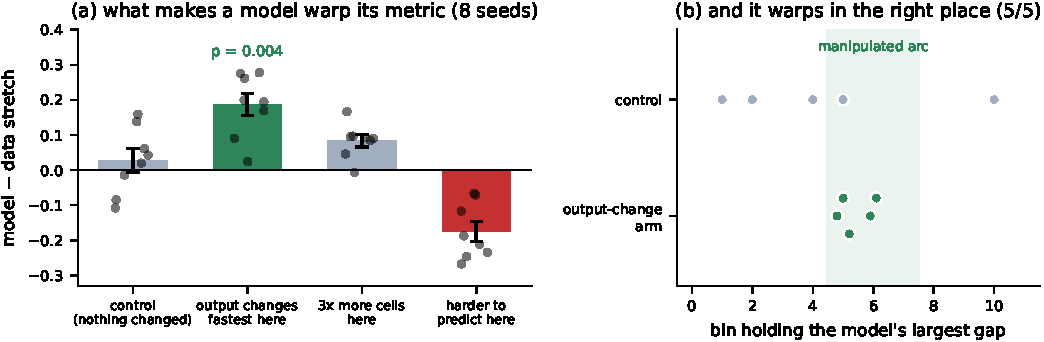
\includegraphics[width=\textwidth]{figures/fig5_warp_law.pdf}
\caption{\textbf{What makes a model warp an inherited metric.} (a) Only the output-change manipulation
separates from control; difficulty produces the opposite sign. Points are individual seeds. (b) The
warp lands inside the manipulated arc in every seed.}
\label{fig:warp}
\end{figure}

\subsection{The gene table is a genuine map, and the model depends on it}\label{sec:table}
The same synthetic setting answers the other open question, which is what a token table is \emph{for},
and whether the chromosome result of \S\ref{sec:add} should have been expected. Assign every gene an
arbitrary group label appearing in \emph{no single cell}, the synthetic analogue of a chromosome, and
sweep how strongly group membership drives co-occurrence. The table tracks a training-free
factorisation across the whole dose-response curve, reaching $0.426$ at full strength against the
factorisation's $0.497$ and a chance rate of $0.050$.
It \textbf{generalises to genes that never co-occur in any cell}, which is the synthetic form of the
neighbourhood holdout, at four times the factorisation's own generalisation (held-out cosine $+0.0147$
against $+0.0037$; Stouffer $z=+20.2$). And \textbf{freezing the table at random initialisation costs a
quarter of the model's performance} (val\_corr $0.853 \to 0.612$), so the structure is load-bearing.
Together these make the real-model chromosome result expected: a token table is where a transformer
puts corpus-level structure, because it is the only component that sees the corpus and not a single
cell.

\subsection{Navigability is decided by topology, not by the model}\label{sec:stall}
The anatomy of \S\ref{sec:inherit} said the cell cycle is a closed loop. That fact alone, before any
question about what the model learned, determines whether the most common steering method can work.

For any closed curve and any fixed direction $\mathbf{w}$,
$\oint \mathbf{w}\cdot d\mathbf{x} = \mathbf{w}\cdot\oint d\mathbf{x} = 0$. A constant-direction
steerer therefore does exactly zero net work per lap. Because the operator unit-normalises each step, a
projected constant direction becomes $\mathrm{sign}(\mathbf{w}\cdot\hat{t})\,\hat{t}$: it advances
while $\mathbf{w}\cdot\hat{t}>0$, retreats once $\mathbf{w}\cdot\hat{t}<0$, and converges to a stall
where $\mathbf{w}\perp\hat{t}$, about a quarter-turn in, \emph{even on a perfectly flat circle}.

Pre-registered, then verified three ways (Fig.~\ref{fig:stall}). Analytically, above. On a synthetic
zero-curvature circle, stall at $1.49$\,rad against the predicted $\pi/2=1.571$, with the
pre-normalisation step norm collapsing to $0.09$ of its initial value, a judge-free measurement of
$\mathbf{w}\perp\hat{t}$. And in seven representations including raw expression with no model at all,
fixed direction $0.01$ to $0.36$ laps against local-tangent $4.5$ to $6.0$. Measured cell by cell, the
phase rate peaks \emph{exactly} at the perpendicular crossing ($90.7^\circ$), banking 55.3\% of total
advance before it. This single fact explains a family of failed steering results at a stroke, and it
explains them without reference to any property of any model: the geometry of the target, rather than
the quality of the representation, was the obstacle.

\begin{figure}[t]
\centering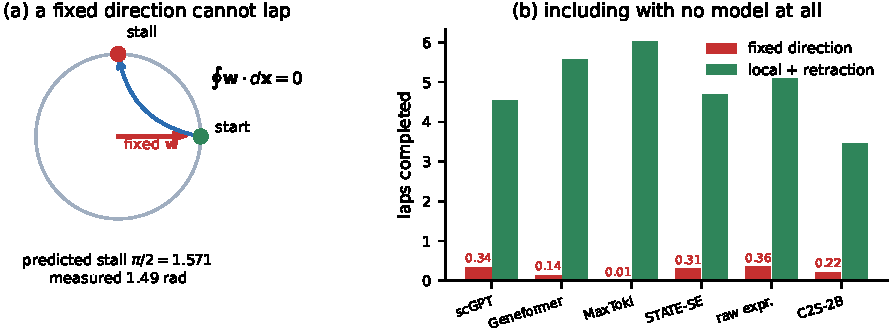
\includegraphics[width=\textwidth]{figures/fig6_stall_theorem.pdf}
\caption{\textbf{Topology, not the model, decides navigability.} (a) A fixed direction does zero net
work per lap and stalls a quarter-turn in. (b) The prediction holds in every representation, including
raw expression.}
\label{fig:stall}
\end{figure}

\subsection{A steering operator that works}\label{sec:operator}
Diagnosing why steering fails is only half of it; the geometry also says what to do instead. The tree
shape of \S\ref{sec:inherit} says the direction must be local, and the stall theorem says the step must
be projected onto the tangent.

\textbf{Local direction $+$ tangent projection $+$ retraction.} On a branching trajectory, keeping one
global direction but re-projecting it at every step onto the top-$m$ right singular vectors of the
$k=100$ nearest real training cells lifts constrained advance from $0.461$ to $\mathbf{1.239}$,
positive in \textbf{16 of 16} model $\times$ tissue cells and beating an oracle allowed to use held-out
labels in 12 of 16. Ablations separate the ingredients: projection alone gives $+0.778$, local
direction alone gives $-0.072$. On a \emph{closed} loop the balance reverses and locality dominates,
which is what the two topologies predict. Retraction cures outward drift but never the stall. The
operator needs only a cell-by-gene matrix, so we release it as a model-free tool.

\textbf{Behaviour follows geometry.} A fitted manifold could be an artefact of the fitting procedure,
so the last check reads the model, not the embedding. Walking a cell state around the fitted
manifold and patching it into a real forward pass drives the model's \emph{own next-gene predictions}
around the cycle: $1.579$ behavioural laps for the local-tangent rule against $0.212$ for a fixed
direction, 12 of 12 cells favouring local-tangent ($p=2.4\times10^{-4}$), with a
representation$\to$behaviour isometry of $0.73$ to $0.88$. The geometry we fitted is the geometry the
model computes with.

\subsection{The geometry arrives bent, and part of the bending is size}\label{sec:curv}
One question remains about where geometry comes from: whether the network builds it with depth, as the
usual framing assumes. It arrives at layer 0 instead, and a large part of what has been measured as
curvature turns out to be vector magnitude. This subsection concerns the \emph{developmental}
trajectory. The cell-cycle loop of \S\ref{sec:inherit} is flat, and there is no conflict: a curve can
bend through a high-dimensional space while a loop lies in a plane, and these are two different
objects measured on two different substrates.

Whether these manifolds actually \emph{bend}, as opposed to a quadratic term merely predicting
pseudotime better than a linear one, was not established before. We separate \textbf{angular} curvature
(real bending) from \textbf{radial} curvature (nonlinearity in vector magnitude, that is, LayerNorm and
scale effects), at matched width across all layers (Table~\ref{tab:curv}, Fig.~\ref{fig:curv}).

\begin{table}[h]\centering\small
\caption{\textbf{Curvature separated into shape and size.} Angular curvature is genuine bending of the
trajectory; radial curvature is nonlinearity in vector magnitude. The ratio column is radial/angular.
``Peak layer'' is the layer at which angular curvature is highest, out of the model's total; in all
three it is the input or the layer next to it. The final column shows how strongly the vector norm
alone tracks pseudotime.}
\label{tab:curv}
\begin{tabular}{lccccc}
\toprule
model & peak layer & angular & radial & ratio & $\mathrm{corr}(\|x\|,\text{pseudotime})$ \\
\midrule
scGPT & \textbf{0} of 11 & $+0.0480$ & $+0.0209$ & $0.44$ & $+0.42$ \\
MaxToki-217M & \textbf{1} of 11 & $+0.0598$ & $+0.0252$ & $0.42$ & $+0.47$ \\
MaxToki-1B & \textbf{0} of 20 & $+0.0552$ & $+0.0050$ & $\mathbf{0.09}$ & $+0.21$ \\
\bottomrule
\end{tabular}
\end{table}

\textbf{The manifold does bend}, since angular curvature clears its null in all three models.
\textbf{But roughly 40\% of the apparent curvature is magnitude rather than shape} in two of three,
where the vector norm itself tracks pseudotime at $+0.42$ and $+0.47$; only the largest model is nearly
pure. Any statistic that fails to separate the two overstates the geometry. And in all three, curvature
\textbf{peaks at layer 0 or 1} and decays with depth, so the manifold \emph{arrives bent} rather than
being constructed. This sits in tension with the common framing of these representations as something
the network builds with depth, and it is consistent with the rest of the paper: the structure comes in
with the data and the embedding table, not from the stack.

\begin{figure}[h]
\centering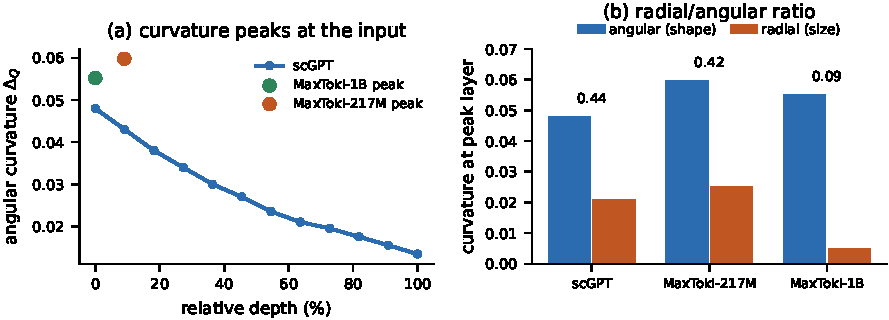
\includegraphics[width=0.92\textwidth]{figures/fig7_curvature.pdf}
\caption{\textbf{Curvature is real, partly radial, and front-loaded.} (a) Angular curvature peaks at or
next to the input in all three models. (b) Two of three are substantially radial, so a statistic that
does not separate shape from size overstates the geometry.}
\label{fig:curv}
\end{figure}

\section{Separating a model's geometry from its input's geometry}\label{sec:controls}

The results above rest on a small set of tests that decide attribution. We state them here as a
protocol, because they are the part of this work most reusable by others, and because each can be
applied to a published claim without rerunning the original study. Each test is paired below with a
measurement showing what it catches.

\paragraph{1. Match the baseline to the model's input, on both encoding and selection.} A baseline is
only a competitor if it holds the same information. In the cross-cell-line transfer of
\S\ref{sec:inherit}, matching the encoding alone yields ``the model adds information'' ($\Delta=+0.0153$,
CI excluding zero), while additionally matching how genes were selected yields parity
($\Delta=-0.0022$) on the same cells.

\paragraph{2. A permutation null says an effect is not noise; only a baseline says it is the model.}
This is the most consequential test and the one most often skipped. In \textbf{six} separate cases here
a large $z$ against a permutation null goes to approximately zero against a competitor built from the
same cells (Supplement~F.3). The most instructive: a label constructed from \emph{pure sampling noise}
scored $0.447$ at $z=35.8$, higher than the real biological label at $0.357$, $z=24.9$. A permutation
null asks whether the labels carry the effect. Attribution asks whether the model does, and only a
competitor can answer that.

\paragraph{3. The baseline panel must express the biology in question.} A baseline built on cells that
do not exhibit the phenomenon measures the panel's blindness rather than the model's skill. HOX genes
are expressed in 3\% of Tabula Sapiens cells, where a co-expression baseline scored $0.08$. The trap
runs in reverse too. On non-proliferating tissue the models score $0.767$ on the cell cycle against a
co-expression baseline's $0.495$; rebuild the same baseline on cycling cells and it gives $0.879$
against MaxToki's $0.358$. The panel, not the model, moved.

\paragraph{4. Make comparisons invariant to orientation, magnitude and width.} Three nuisance
quantities masquerade as structure. \emph{Orientation}: in cross-tissue transfer an apparent model
advantage of $+0.278$ ($p=0.016$) falls to $+0.094$ ($p=0.23$) once the comparison is made invariant to
the arbitrary sign of each tissue's pseudotime; the advantage was consistency of direction, not
structure. \emph{Magnitude}: roughly 40\% of measured curvature is vector norm (\S\ref{sec:shape}).
\emph{Width}: comparing representations at native dimensionality measures width as much as content, and
reducing MaxToki-1B from 2{,}304 to 256 components costs nothing at layer 0 ($0.910 \to 0.813$) while
collapsing layer 8 ($0.265 \to 0.066$).

\paragraph{5. Score two nulls against each other before reporting an effect against one.} If an
estimator is biased, a null-versus-null comparison reveals it while a null-versus-real comparison hides
it. One estimator here returns $-0.489$ comparing two structureless labellings against each other,
larger in magnitude than the $-0.227$ it returns on the real comparison, so its output on the real
comparison carries no information and the arm is not reportable (Supplement~D.4).

\paragraph{6. Report readable, model-specific and used separately.} Each of the three can hold without
the others, so none of them implies another, and our data contain a worked case of every dissociation
we could measure. \emph{Used but not model-specific:} a
functional-context axis is causally used at $p=4.3\times10^{-7}$ (signed swing $+0.815$, 28 of 30
cells, dose-monotone) yet fails its co-expression-coherence null at $+1.16\sigma$. \emph{Readable but
not used:} sub-chromosomal position decodes at $\rho=+0.396$ in 22 of 22 chromosomes and beats both
baselines, yet the causal response is flat along the chromosome. \emph{Readable but not traversable:}
cell-cycle phase reads at $0.93$ from gene tokens while the geometry is a two-pole axis with minimum
angular gap $1.6$ to $30.7^\circ$, against $90^\circ$ for a real circle.

\paragraph{A note on extraction.} Two data defects, both found here, both biasing in a known direction,
are worth flagging for anyone using the same public assets. Feeding raw counts to a checkpoint
configured for binned input \emph{understates the model and overstates its curvature}: correcting it
raises pseudotime decodability by $0.109$ and linear fit by $0.210$, and \emph{lowers} the measured
curvature gap by $0.075$. And in one widely used cached developmental dataset, differentiated cells sit
\emph{below} stem cells in pseudotime.

These tests are not gentle, and the first result we put through them was one of our own. A
previously reported developmental representation extracted from a frozen model
\citep{kendiukhov2026hematopoietic}, benchmarked against scVI \citep{lopez2018scvi}, Palantir
\citep{setty2019palantir}, DPT \citep{haghverdi2016dpt}, CellTypist \citep{dominguezconde2022celltypist},
PCA and raw expression across 88 donor-holdout splits, does not survive them: the exported operator
performs the same as a \emph{random matrix on the same support} at every bottleneck width ${\ge}10$,
and the model's own frozen representations lose to a dimension-matched \emph{random projection of raw
genes} by $0.0507$ AUROC on \textbf{14 of 14} donors ($p=0.0001$). Every check in the original was
passed; none of those checks was a matched competitor. Supplement~E gives the full battery.

\section{Related work}

Three literatures meet here: what latent variables neural networks build, what geometry has been
claimed for biological foundation models, and how those models fare against simple baselines. Our
position in each follows from the split of \S\ref{sec:inherit} and \S\ref{sec:add}.

\textbf{Emergent world variables.} Board state in Othello \citep{li2023othello,nanda2023linear} and
chess \citep{karvonen2024chess}, look-ahead \citep{jenner2024lookahead}, and space and time in language
models \citep{gurnee2024spacetime} establish that models trained on narrow objectives build
representations of structure they were never taught; the form such variables take, including the
circular features that motivate \S\ref{sec:inherit}, is itself an active question
\citep{engels2025circular,park2024linear}, as is how sharply a model's output responds to movement
between inputs \citep{shinkle2025plateaus}. All of these variables are dynamic and determined by the
current input, and \S\ref{sec:add} argues that vocabulary-level facts are a distinct class.

\textbf{Where a model's geometry comes from.} The closest work to ours is
\citet{prieto2026correlations}, and our results are best read as building on it. They study
superposition in a controlled autoencoder over bag-of-words text and show that when features are
correlated the interference between them can be constructive: the model arranges features by
co-activation, which produces semantic clusters and the cyclical structures reported in real language
models. Their months-of-the-year circle is recovered from a PCA of the data as well as from a PCA of
the weights, so the circle is inherited from the corpus covariance. We reach the same verdict about a
periodic structure in a different domain (\S\ref{sec:inherit}), and extend it three ways. First, the
evidence is a competition instead of a correspondence: our baselines are given \emph{exactly} the
model's own input, which the explicit tokenisation of a cell-sentence model makes constructible, and we
turn that comparison into a protocol (\S\ref{sec:controls}). Second, we add interventions read through
the model's native head and an externally measured ground truth, neither of which is available for
text. Third, two of our findings fall outside their two categories of correlation-driven and
task-driven geometry: a metric that a model reshapes on top of an inherited shape (\S\ref{sec:warp}),
and facts that no single input contains at all (\S\ref{sec:add}). Their closing question, how to
separate these effects in realistic settings, is the question \S\ref{sec:controls} answers.

\textbf{Geometry in biological foundation models.} Low-dimensional cell-state structure is reported by
the model papers themselves \citep{cui2024scgpt,theodoris2023geneformer,rosen2026uce} and analysed
spectrally in our earlier work \citep{kendiukhov2026spectral}, generally as encoding results without a
causal test, and generally without a competitor built from the same data. Reports of gene embeddings
reflecting genomic organisation are local, pairwise and correlational, without neighbourhood holdout or
intervention. Our reading of that literature is the one stated in \S\ref{sec:controls}: absent a
matched competitor, such reports characterise the data as much as the model.

\textbf{Evaluation of single-cell foundation models.} Zero-shot studies question how much these models
add over simple baselines \citep{kedzierska2025zeroshot,boiarsky2023deepdive}, linear baselines match
deep models on perturbation prediction \citep{ahlmanneltze2025linear}, benchmark rankings are unstable
under protocol choices \citep{kendiukhov2026ranking}, attention-derived scores largely re-encode
co-expression \citep{kendiukhov2026attention}, and a protein language model already supplies part of
what single-cell pretraining is credited with \citep{kendiukhov2026twoaxes}. That baselines are competitive is already
established. Our contribution is the split: baselines win on cell state, the model wins outright on
vocabulary facts. To that we add a mechanism for the geometry and a protocol for attributing it.

\textbf{Factorisation baselines.} Skip-gram is implicitly a factorisation of a shifted PMI matrix
\citep{levy2014factorization}, so linear recoverability from a co-occurrence embedding is not by itself
evidence of going beyond co-occurrence. Our label-free retrieval result is consistent with that
caution.

\section{Discussion}

\textbf{The boundary.} A model can only add information its input does not already determine. In
single-cell models that boundary falls between the cell and the gene, and it is sharp. Cell-level
geometry loses to matched baselines on every axis we could measure, while gene-level tables carry facts
no cell contains and act on them. The three parts of this paper are one argument: the boundary explains
which geometries are inherited, the warp law explains what a model does to an inherited geometry when
it does modify one, and the topology results explain what can be done with either.

\textbf{In practice.} Cell embeddings should not be expected to outperform careful expression
baselines, and where they are used, the baseline must be given the model's own input. Gene-embedding
tables are the component worth mining, and the neighbourhood holdout is the control that makes such
claims credible. Because these tables encode chromosome, any comparison between groups differing in
karyotype, such as tumour against normal or aneuploid disease states, inherits a confound that should
be regressed out rather than assumed absent.

\textbf{Limitations.} The chromosome result clears its strongest baseline only in the larger of two
checkpoints, inverts under a label-free test, and the baseline's own score varies sixfold across tissue
panels for reasons we have not explained; the decisive control, scoring against Hi-C compartments and
replication timing, is not yet run. Cross-tissue transfer is measured on six usable pairs. The
synthetic work uses small models on simple planted structures. Attention was measured for chromosome
but not for the cell cycle. The two extraction defects above are documented but not yet corrected
across all affected analyses.

\textbf{Single-cell models as a test bed for questions about language models.} The questions asked here
are not specific to biology. How a low-dimensional geometry forms in a trained network, when a model
reshapes a metric it inherited, what a token table stores, and which steering operations a topology
permits were all asked of language models first, and are hard to settle there. A single-cell model is a
smaller and more tractable place to ask them, for three reasons that recur throughout this paper. Its
input is a vector of numbers, so a competitor holding \emph{exactly} the model's own input can be
constructed, which is what made the accounting in \S\ref{sec:inherit} possible and is rarely available
for text. Its vocabulary is fixed, finite and externally annotated, so a claim about what a token
embedding knows can be checked against a genome instead of against intuition. And its ground truth is
independently measurable: the cell cycle is periodic, genes sit where the assembly says they sit, and a
karyotype can be measured without reference to any model. Several results here have direct counterparts
in the language-model literature, including a circular representation of a periodic variable, a latent
world variable that no single input contains, and the failure of a fixed steering direction on a closed
feature. Where the counterparts differ they differ informatively, as with the continuity result of
\S\ref{sec:inherit}. \citet{prieto2026correlations} close by asking how to separate data-driven from
task-driven geometry in more realistic settings than a controlled autoencoder allows; a single-cell
model is such a setting, and \S\ref{sec:controls} is our answer to that question. We suggest treating
these models as a controlled place in which claims about representational geometry can be tested more
cheaply and more decisively, with the conclusions carried back.

\paragraph{Code and data.} Everything is at
\url{https://github.com/Biodyn-AI/geometry-sc-models}: the analysis code organised by the section it
supports, an index mapping every claim to the script that produced it, the figure scripts, and about
280 result files committed beside the code that wrote them, so any number here can be checked without
rerunning anything. The synthetic programme of \S\ref{sec:warp} and \S\ref{sec:table} runs end to
end with no external assets. Model checkpoints and datasets are third-party and are not
redistributed; the repository documents each one and where to obtain it. The steering operator of
\S\ref{sec:operator} is released as a standalone tool requiring only a cell-by-gene matrix.
Experiments that failed, including the two whose instruments proved untrustworthy, are included
deliberately.

\bibliographystyle{unsrtnat}
\bibliography{refs}

% ===================================================================
%  Supplementary Material
% ===================================================================
\clearpage
\setcounter{secnumdepth}{0}
\setcounter{page}{1}
\renewcommand{\thepage}{S\arabic{page}}
\begin{center}
{\LARGE\bfseries Supplementary Material}
\end{center}
\vspace{2pt}

{\small
\input{supplement_body}
}

\end{document}
